This section describes the software that we used, a class diagram of our implementation and a flow chart of how the robot interacts with its environment.

\subsection{Software used}
The robot needs to execute multiple tasks and react on many inputs at once. Therefore we were recomended to use Robot Operating System (ROS) which is a software framework that can be run on other *nix-like operating systems like GNU/Linux and Mac OS X. ROS basically works as a intermediate ``talker'' between the different processes that we run on our robot. The advantage of using ROS instead of explicitally create threads that can comunicate with each other is that we can rather simple separate each functionality and test them seperately. It also unsure that we don't need to handle deadlocks and shared objects. The drawbacks are the time it takes to get a good grep of how ROS works, and that it has a slight overhead compared to pthread library.

Other software that we used were:
\begin{itemize}
\item Git for version controlling.
\item Gcc for compiling our C-code.
\item Python 2.7 for running some scripts and for map visualization.
\item OpenCV for computer vision.
\item Google Sketchup for drawing 3D models.
\item Fabric, a python library, for copying binany files from the workstation to the robot.
\end{itemize}

\subsection{Software Structure}
We started to implement some highlevel part (MovementController) in python, but later found out that it was too slow to run on the hardware that we currently have. By translating the code directly to C++, we could see a huge difference in performance.

Through the whole project, we had to restructure our code multiple times. This was partly because we did not know what problem we could encounter. For example we had to add many movement states for the robot to handle all the type of movements that we had not thought of.

Below you can see a flowchart of the final implementation.

\begin{figure}[h!]
\label{fig:flow_chart}
    \begin{centering}
   	 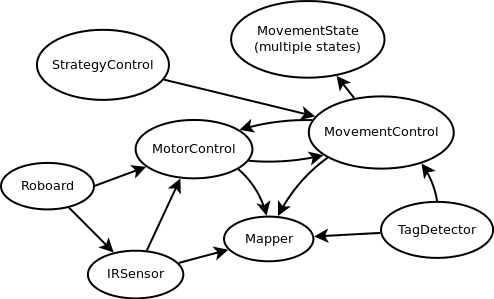
\includegraphics[scale=0.5]{figures/flow_chart.png}
   	 \caption{A flow chart of how the different processes interact}\label{fig:flow_chart}
    \end{centering}
\end{figure}

